\newcommand{\piston}{
  \begin{figure}
    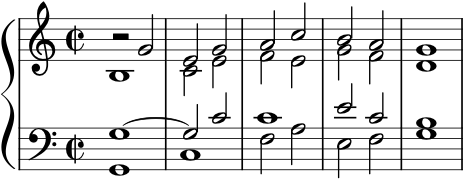
\includegraphics[width=6cm]{fig/piston1.png}
    \caption{Piston Harmonization}
    \label{fig:piston}
  \end{figure}
}

\newcommand{\fharm}{
  \begin{figure}
    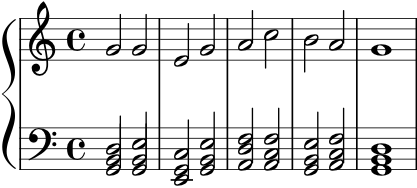
\includegraphics[width=6cm]{fig/piston2.png}
    \caption{FHARM Harmonization}
    \label{fig:fharm}
  \end{figure}
}

\section{Harmony}
\label{sec:harmony}

TODO: Harmonize melody, use counterpoint for voice leading and to contrain harmony.
Mention grid for harmonic analsis, makes use of vectors.

\piston

\fharm
